\documentclass{beamer}

\mode<presentation>{\usetheme{poster}}

% Load packages here
\usepackage{amsmath,amssymb,array}
\usepackage{graphicx,tcolorbox}
\usepackage{ragged2e}
\tcbuselibrary{listings,breakable,most,hooks,skins}
\graphicspath{{./graphics/}}
\usepackage[orientation=landscape,size=custom,width=48,height=36,scale=.6,debug]{beamerposter}
\usepackage{mathptmx}
\usepackage{verbatim}
\renewcommand\sfdefault{ptm}
\def\Z{\mathbb Z}
\def\N{\mathbb N}
\def\Q{\mathbb Q}
\def\R{\mathbb R}
\def\C{\mathbb C}

% Header and footer 
\newcommand{\footleft}{http://mcl.math.uic.edu/}
\newcommand{\footright}{}
\title{Vietoris-Rips complexes, random points on varieties, and persistent homology}
\author{Mason Boeman \quad Daniel Etrata}
\institute{Mentors: Benjamin Antieau and J\={a}nis Lazovskis}

% Main document
\begin{document}
\begin{frame}{}
\begin{columns}[t]

%-- Column 1 ---------------------------------------------------
\begin{column}{0.32\linewidth}

%-- Block 1-1
\begin{block}{Summary}

The project takes a variety of n-dimensions intersected by random lines to generate points. From this point cloud, an undirected neighborhood graph is constructed,
where the edges are assigned a weight. Then, the neighborhood graph undergoes the Vietoris-Rips expansion by constructing cofaces for which the vertex is maximal.
\end{block}



%-- Block 1-2
\begin{block}{Motivation}
The goal of this project is to use persistent homology to study the topology of random complex algebraic varieties,
geometric figures described as the solution sets of system of polynomial equations. 

\end{block}

%-- Block 1-3
\begin{block}{Using PHCpack to find points}
PHCpack is a polynomial system solver using homotopy continuation methods [1]. Let $f(x) = 0$ be the target system. PHC constructs $g(x)=0$ start system. Then let $\gamma$ be the accessibility constant, $\gamma \in \C$ and $t$ be the continuation parameter, $t \in [0,1]$. The homotopy $h$ is defined as
\begin{equation*}
h(x,t) = \gamma \cdot (1-t)\cdot g(x) + t \cdot f(x) = 0
\end{equation*}
\begin{equation*}
h(x, 0) =g(x)
\end{equation*}
\begin{equation*}
h(x, 1) = f(x)
\end{equation*}
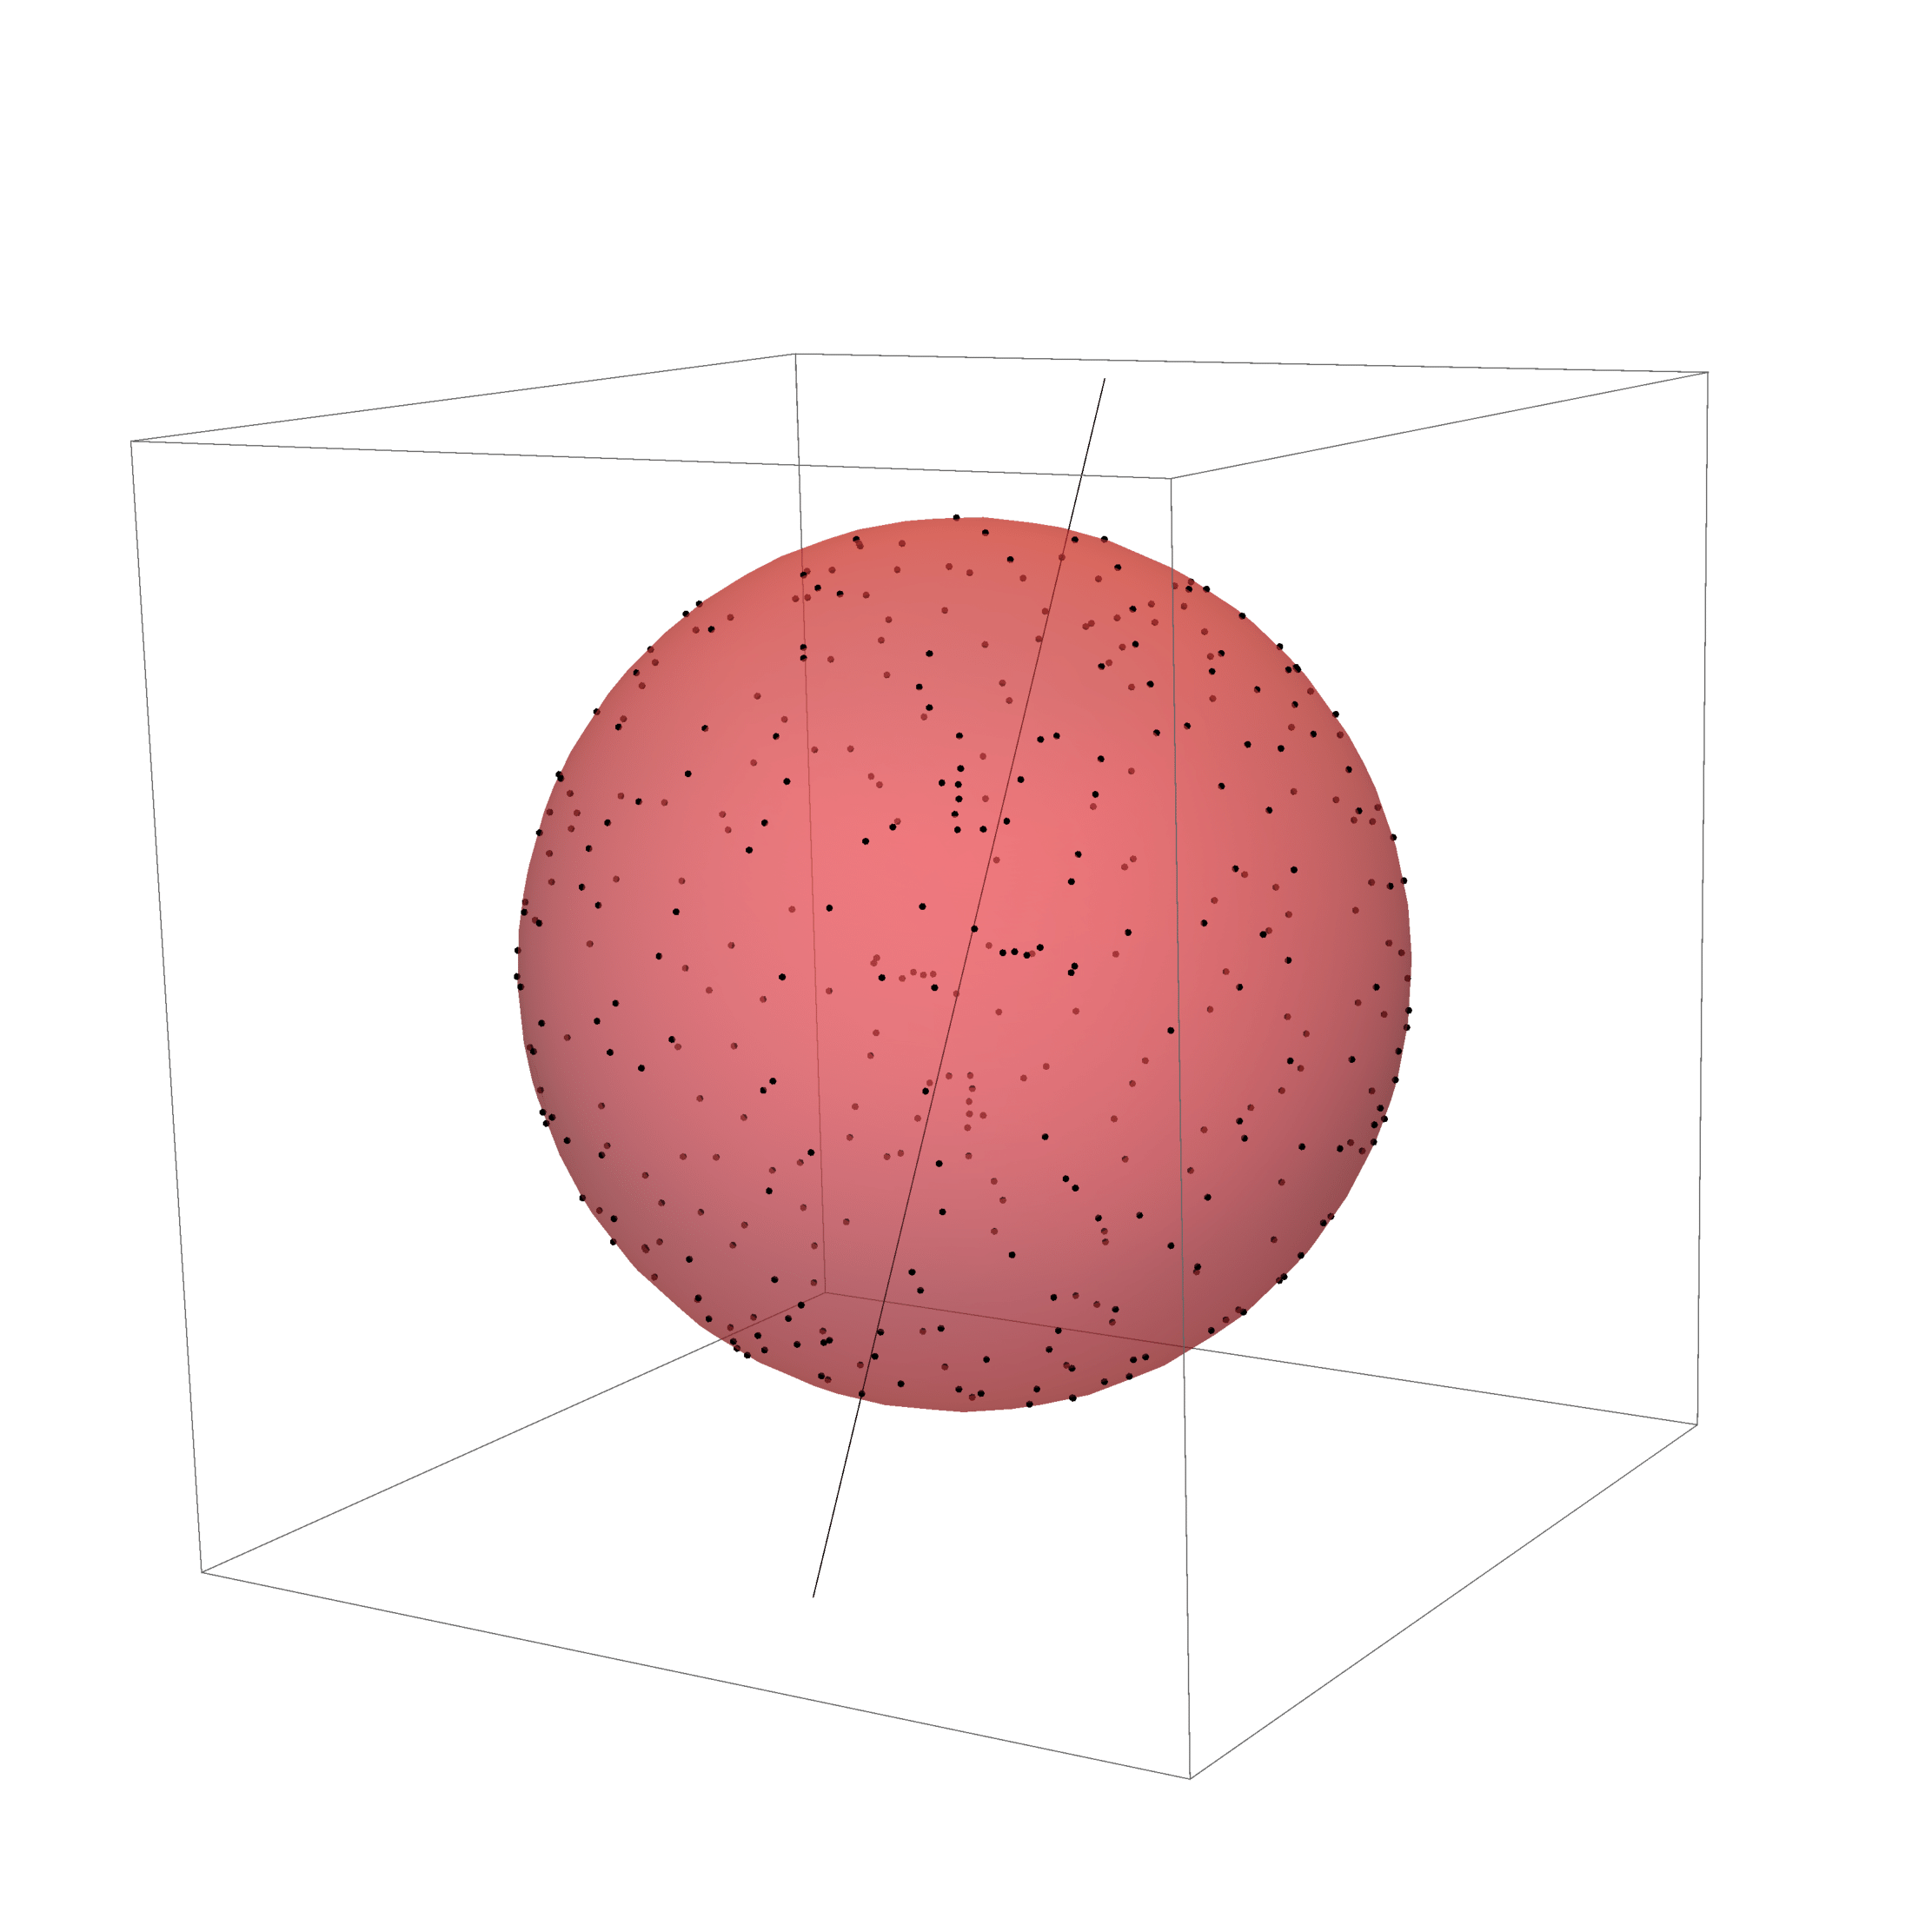
\includegraphics[width=.5\columnwidth]{sphere-1}
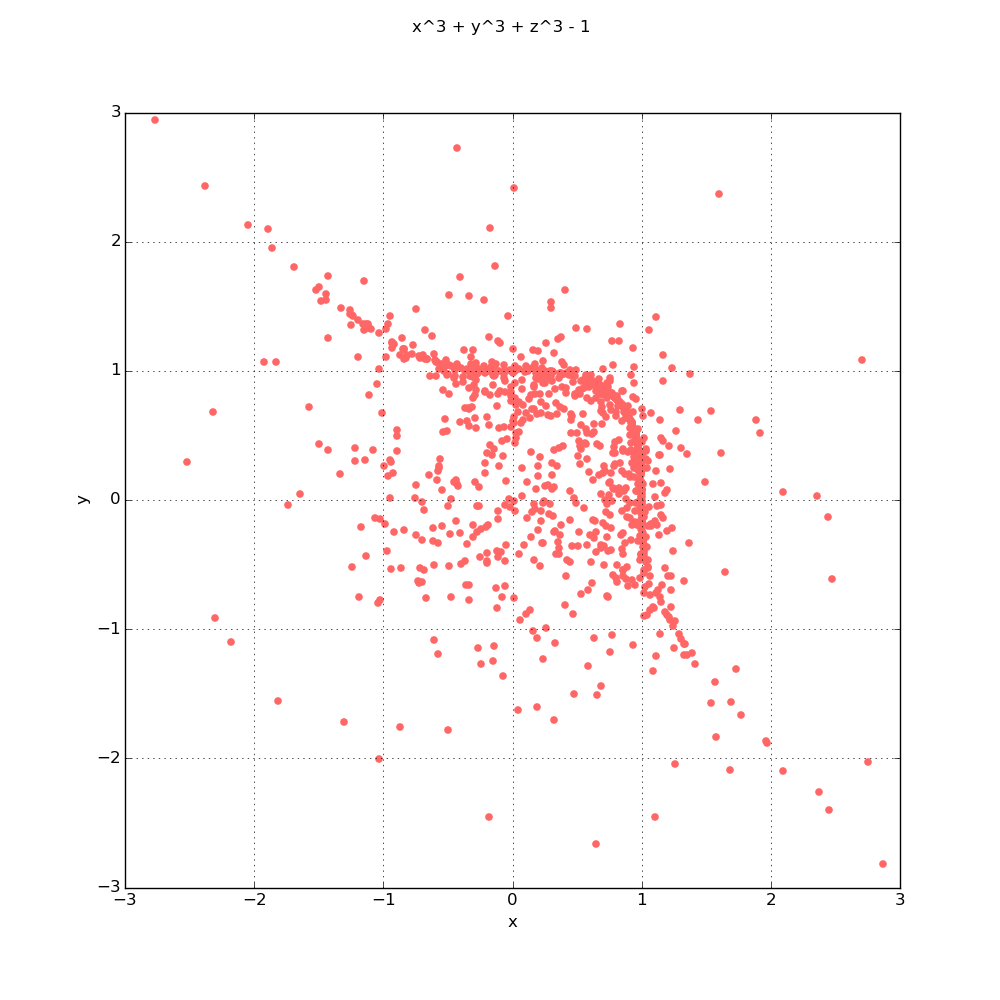
\includegraphics[width=.5\columnwidth]{plot2d_5}


\end{block}


\end{column}%1

%-- Column 2 ---------------------------------------------------
\begin{column}{0.32\linewidth}

%-- Block 2-1
\begin{block}{Neighborhood graphs}

The neighborhood graph of a set $S$ with a parameter $\epsilon$ is the graph
with vertices in $S$, where an edge is contained in the neighborhood graph if
and only if the distance between it's endpoints is less than $\epsilon$. Our
quick edge algorithm takes as input a set of points $S$ of order $n$ in affine
space, and some positive real number $\epsilon$, and produces a list of all edges that have length less than $\epsilon$. Our method uses recursion. If our ambient space has dimension $d$, let $k$ be some positive integer less than $d$. 
\\

First we compute the median value of the $k$-th coordinate of all the points in $S$, and call this $m$. Now we construct four subsets of $S$: $A$, $B$, $A^*$, and $B^*$. $A$ is the set of points whose $k$-th coordinate is less than $m$. $B$ is defined as $S-A$. $A^*$ and $B^*$ are subsets of $A$ and $B$ respectively where points in these sets have kth coordinate within $\epsilon$ of $m$. We add an edge to our list for every pair $(a,b)$ where $a$ in $A^*$ and $b$ in $B^*$, and they are within $\epsilon$ of each other. We then call the algorithm recursively, replacing $S$ with $A$ and $B$, each half the size.

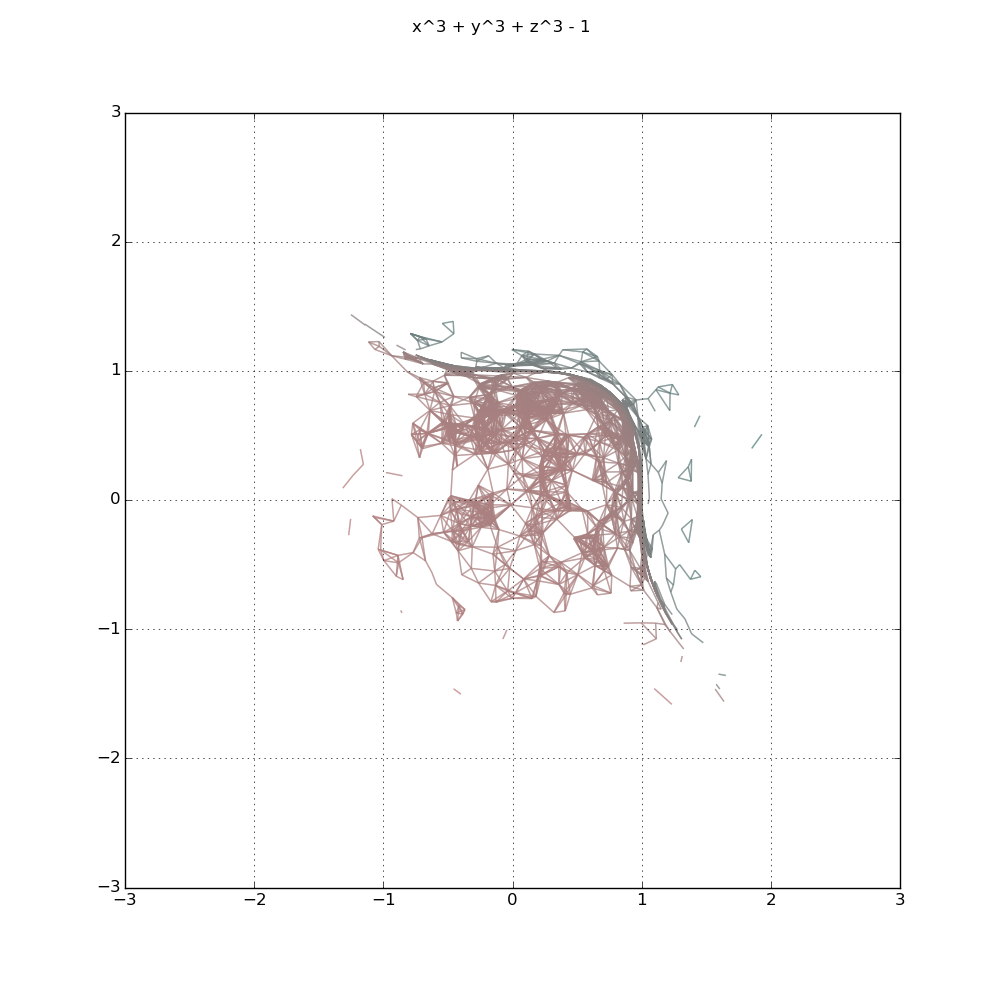
\includegraphics[width=1\columnwidth]{plot2d_ng_7}
\end{block}

\end{column}%2

%-- Column 3 ---------------------------------------------------
\begin{column}{0.32\linewidth}

%-- Block 3-1
\begin{block}{Some connectivity tests}
\includegraphics[width=1\columnwidth]{23plots.png}
\end{block}



%-- Block 3-2
\begin{block}{Persistence and future work}

In the future, we would like to conduct a more thorough test relating
connectivity, number of points, and the size of coefficients. In particular, we
are interested in whether the sharp-threshold phenomenon found in random graphs
can be detected in random points of algebraic varieties.

The main future goal is to fully implement a persistence package that makes it
possible to study the betti numbers of random algebraic varieties.

\end{block}
%-- Block 3-3
\begin{block}{Citations}
\hangindent1em
\hangafter=1
[1] Verschelde, J. (1999). "PHCpack: a general-purpose solver for polynomial systems by homotopy continuation.'' Algorithm 795 in  ACM Trans. Math. Softw. 

%\hangindent1em
%\hangafter=1
%[2] Zomorodian, A. (2010). "Fast Construction of the Vietoris-Rips Complex." Computers \& Graphics, 34.3.

\end{block}

%-- Block 3-4
\begin{block}{Another pretty picture}
Below we show the neighborhood graph with $\epsilon=.2$ associated to $5000$
random points on the torus. In this picture there are 17 connected components.

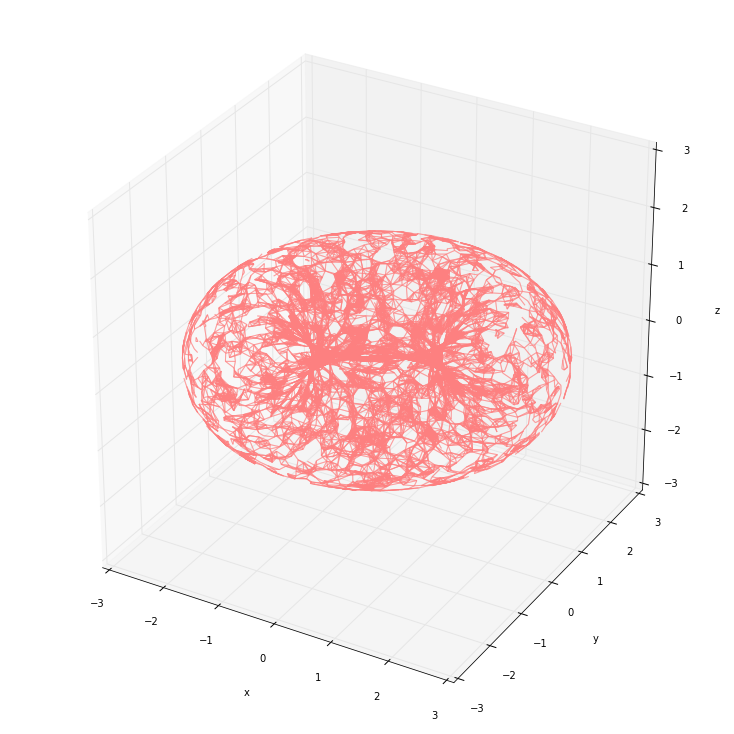
\includegraphics[width=1\columnwidth]{torus.png}

\end{block}

\end{column}%3

\end{columns}
\end{frame}
\end{document}
